\section{Taxonomy}
\label{sec:terminologies}

This section defines common terminologies that are used throughout the paper.

\subsection{From raw data to bit streams}

Our goal is to introduce the concept of resolution and precision to data stored as a simple grid.
For resolution, we use the discrete wavelet transform, in particular, the popular CDF5/3 [CITE]
transform. For precision, we quantize the floating-point wavelet coefficients to $16$-bit signed
integers, thereby eliminating the exponent bits so that every bit can be associated with a bit
plane. To further avoid special treatment of the sign bit in two's complement form, we convert the
quantized coefficients to negabinary form [CITE]. This transformation increase the number of bit
planes from $16$ to $17$.

In practice, bits are never read and transmitted one by one, so in this paper, our fundamental unit
of data is a \emph{chunk} of bits. A \emph{chunks} is a bit plane of a group of $4\times 4$
coefficients in the same subband (the multi-dimensional wavelet transform rearranges the
coefficients into subbands [CITE], each can be thought of as a resolution level). Each group hence
contains $17$ chunks. For all the experiments in this paper, we perform the wavelet transform $3$
times in each dimension, producing $10$ subbands in 2D and $22$ subbands in 3D. Figure
\ref{fig:pipeline} illustrates how all these steps fit together to produce a stream of chunks from
the original, raw data.

\begin{figure}
  \centering
  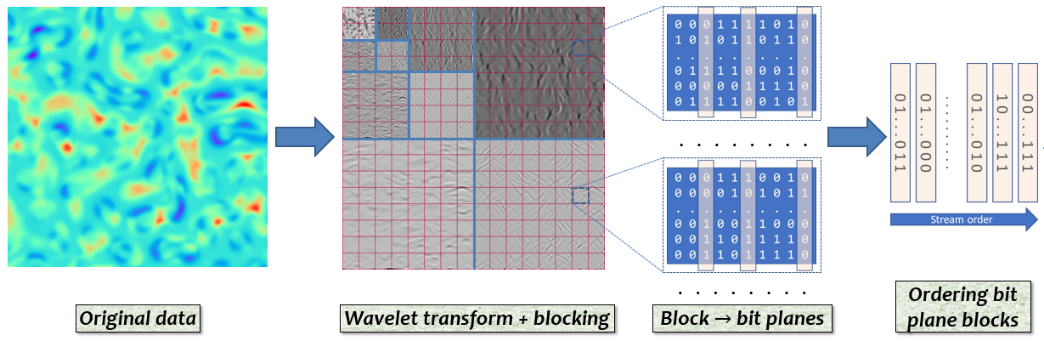
\includegraphics[width=\linewidth]{img/pipeline.png}
  \caption{Our data stream creation pipeline. The input is a regular grid, the output is a stream of
  chunks, where each chunk is a bit plane from a group of quantized wavelet coefficients stored in
  negabinary format. The subbands are separated by blue lines in the second image, with the coarsest
  subband at the top left corner. TODO: revise this figure}
  \label{fig:pipeline}
\end{figure}

\subsection{Static and dynamic streams}
\label{sec:static-dynamic-streams}

In our data streaming model, there is a ``server'' which serves data and a ``client'' which requests
for and receives data from the server. Although the server and the client can both be on the same
machine physically, the server has full knowledge of the data, while the client does not. Thus, when
the client receives a bit, it might not know where the bit should be deposited. A solution to this
problem is to have both the client and the server agree on an ordering of bit positions beforehand.
We use the term \emph{static stream} to refer to streams using this solution. In constrast, a
\emph{dynamic stream} is one in which the client is assumed to ``magically'' know the positions of
the bits without any prior agreement with the server. Dynamic streams have an advantage over static
streams in that they can make use of bit values, not just their positions, to better prioritize the
important bits. However, this also means that dynamic streams are ill-suited for practical
implementations, because the cost associated with streaming bit positions likely outweights any
potential benefit.

In this paper, we use the terms \emph{by bit plane}, \emph{by level}, and \emph{by wavelet norm} to
refer to three common static bit orderings (their exact definitions are in Section [REF]). In
addition, we also consider a \emph{signature}-based stream (Section \ref{sec:stream-signature}) to
be static. This is becaue, in a signature-based stream, the server and the client established the
agreement over bit positions over the transmission of a negligibly small message, called signature,
before any actual value bits are transmitted. As we will show throughout the paper, the use of such
signatures can sometimes result in significant improvements over using purely static streams.

\subsection{Common static streams}
A bit stream can be viewed as a collection of bits, sorted by some weight associated with each bit.
In the literature, two of the most common orderings of bits are \emph{by level} and \emph{by bit
plane}. The \emph{by level} stream orders the chunks strictly from coarser to finer resolution
levels. The weight function used by this stream is $W_1(c)=\bar{l}-L(c)$, where $L$ is a function
that returns the subband (resolution level) of its argument (higher-numbered subbands are finer),
and $\bar{l}$ is the total number of subbands. Within the same subband, without any further
knowledge of the underlying data, the chunks naturally follow the row-major order. The second common
stream, \emph{by bit plane}, proceeds stricly from higher-ordered to lower-ordered bit planes (i.e.,
$W_2(c)=\bar{b}-B(c)$, where $B$ is a function that map its argument to the corresponding bit plane
and $\bar{b}$ is the total number of bit planes, with $0$ being the most significant bit plane). 

The \emph{by level} and \emph{by bit plane} streams are designed to mimic the way data is read in
traditional data reduction methods that work either in resolution or in precision space. In this
paper we also define the \emph{by wavelet norm} stream which combines these two dimensions. \emph{by
wavelet norm} orders chunks using $W_3(c)=2^{\bar{b}-1-B(c)}\times \norm{\omega_{L(c)}}^2$. The term
$2^{\bar{b}-1-B(c)}$ captures the contribution of a bit on bit plane $B(c)$, while the term
$\norm{\omega_{L(c)}}^2$ captures the contribution of a coefficient on subband $L(c)$, where
$\omega_{L(c)}$ refers to the wavelet basis function on subband $L(c)$. Note that all three streams
mentioned so far are data-agnostic.

TODO: mention that all streams are without leading zero bits

\subsection{Stream signatures}
\label{sec:stream-signature}

To analyze the core characteristics of a stream, we introduce the concept of a stream
\emph{signature}. A signature is a $B \times L$ matrix, with $B$ being the number of bit planes, and
$S$ being the number of subbands produced by the wavelet transform. A chunk on subband $s$ and bit
plane $b$ can be associated with the $b, l$ cell of the matrix. Every chunk in the stream can be
associated with one (and only one) of the cells. Each matrix cell $(b,l)$ contains a value in the
range of $[0,B\times L)$, indicating the position in which chunks of that cell appear in the stream,
relative to chunks of all other cells, on average. It is our hypothesis that streams optimized for
different analysis tasks produce qualitatively distinctive signatures, and therefore, a set of
signatures can be pre-computed once and later picked to use depending on the analysis at hand.

To compute a stream signature, we partition the whole domain into several regions, compute one
chunks in each per-region signature are spatially related. The reason for this partitioning is that
it is only meaningful to study the relative ordering of cells if the chunks associated with those
cells all come from same region of the original domain. Ideally the global signature for a stream
should contain all the per-region signatures, but due to space constraint, as well as for ease of
visualization, we condense all the local signatures by averaging them on a per-cell basis, and only
study the average signature. (TODO: add the algorithm).

% \begin{algorithm}
%   \KwData{this text}
%   \KwResult{how to write algorithm with \LaTeX2e }
%   initialization\;
%   \While{not at end of this document}{
%    read current\;
%    \eIf{understand}{
%     go to next section\;
%     current section becomes this one\;
%     }{
%     go back to the beginning of current section\;
%    }
%   }
%   \caption{How to write algorithms}
% \end{algorithm}
